\section{Synthesising Configurations across Multiple Domains}
\label{sec:synth-multi}

In this section, we present an algorithm for 
solving the path-compliance problem in the presence
of multiple domains---i.e., $|\{\Theta(r) \mid r\in V\}|>1$.
However, we assume that the domain splitting $\Theta$ is given to us.
Formally, we are given a set of paths $\Pi$,
a topology $T=(V,E)$,
a domain-assignment function $\Theta$, 
and we want to find functions
$LP$, $W$, and $RF$,  such that
$C=(T,W,RF,LP,\Theta)$ and
$\paths^C(PC) = \Pi$..
We call this problem the \emph{inter-domain synthesis problem}.

\subsection{Hard Constraints}
\begin{figure*}
	\centering
	\subfloat[Ex1]{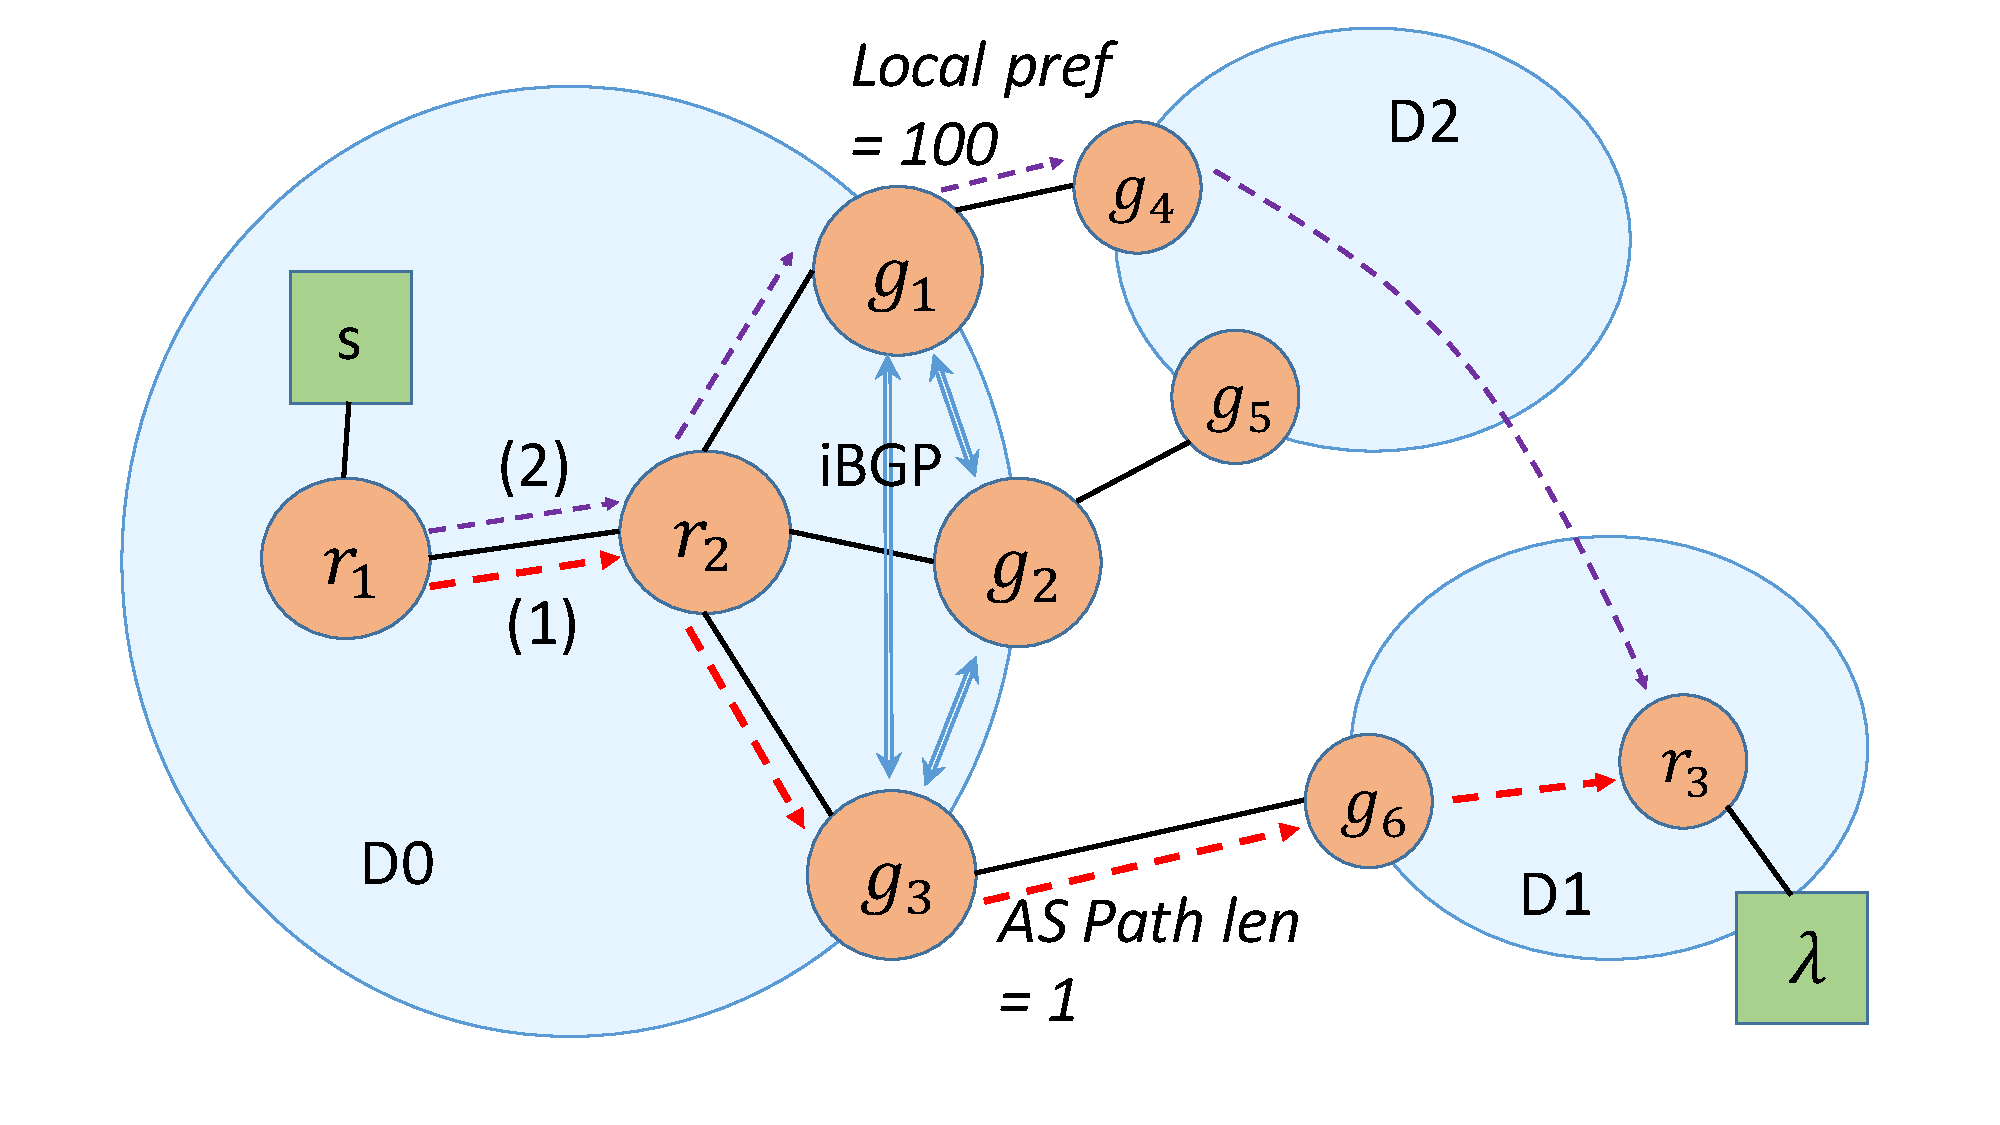
\includegraphics[width=0.66\columnwidth]{figures/bgp-example.pdf}}
	\subfloat[Ex2]{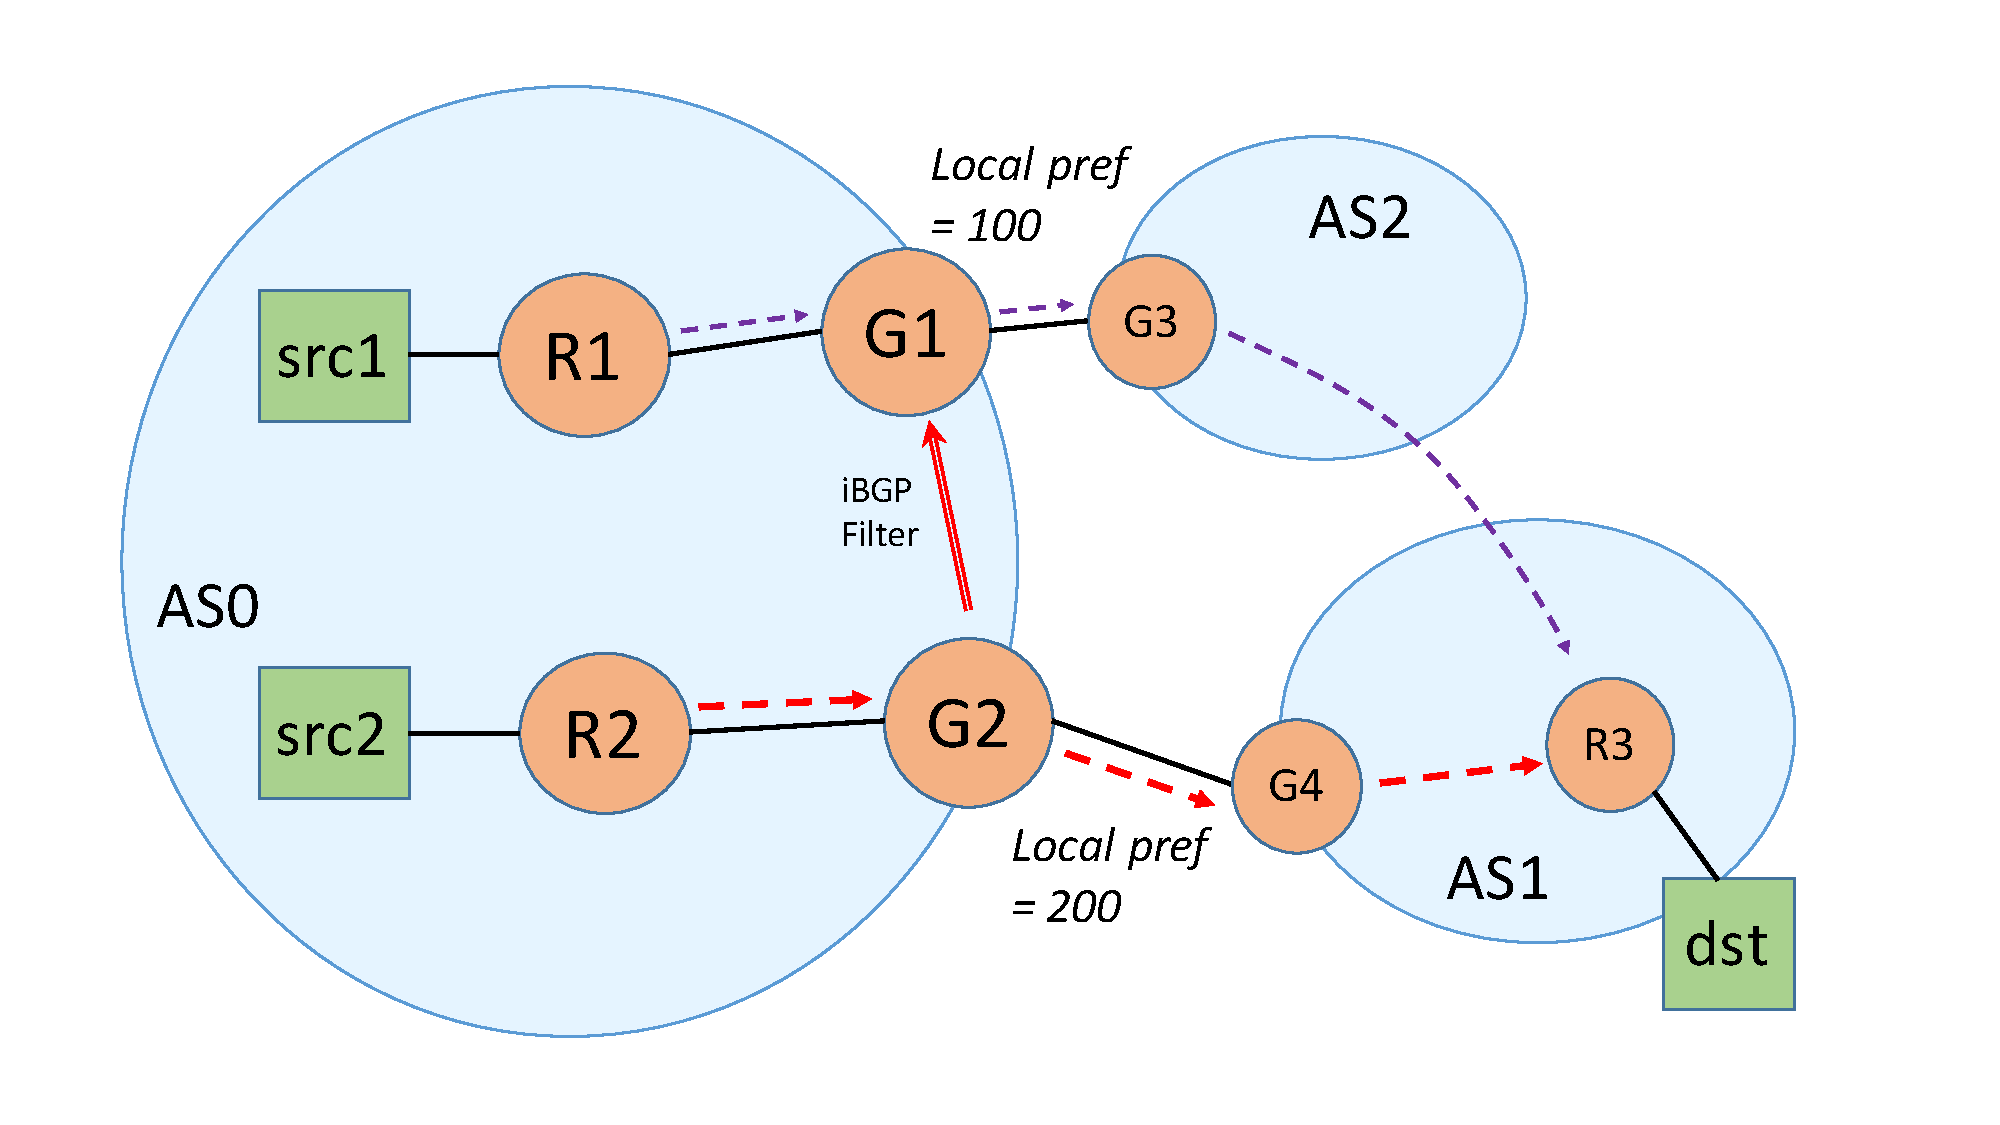
\includegraphics[width=0.6\columnwidth]{figures/bgp-example2.pdf}}
	\subfloat[Ex3]{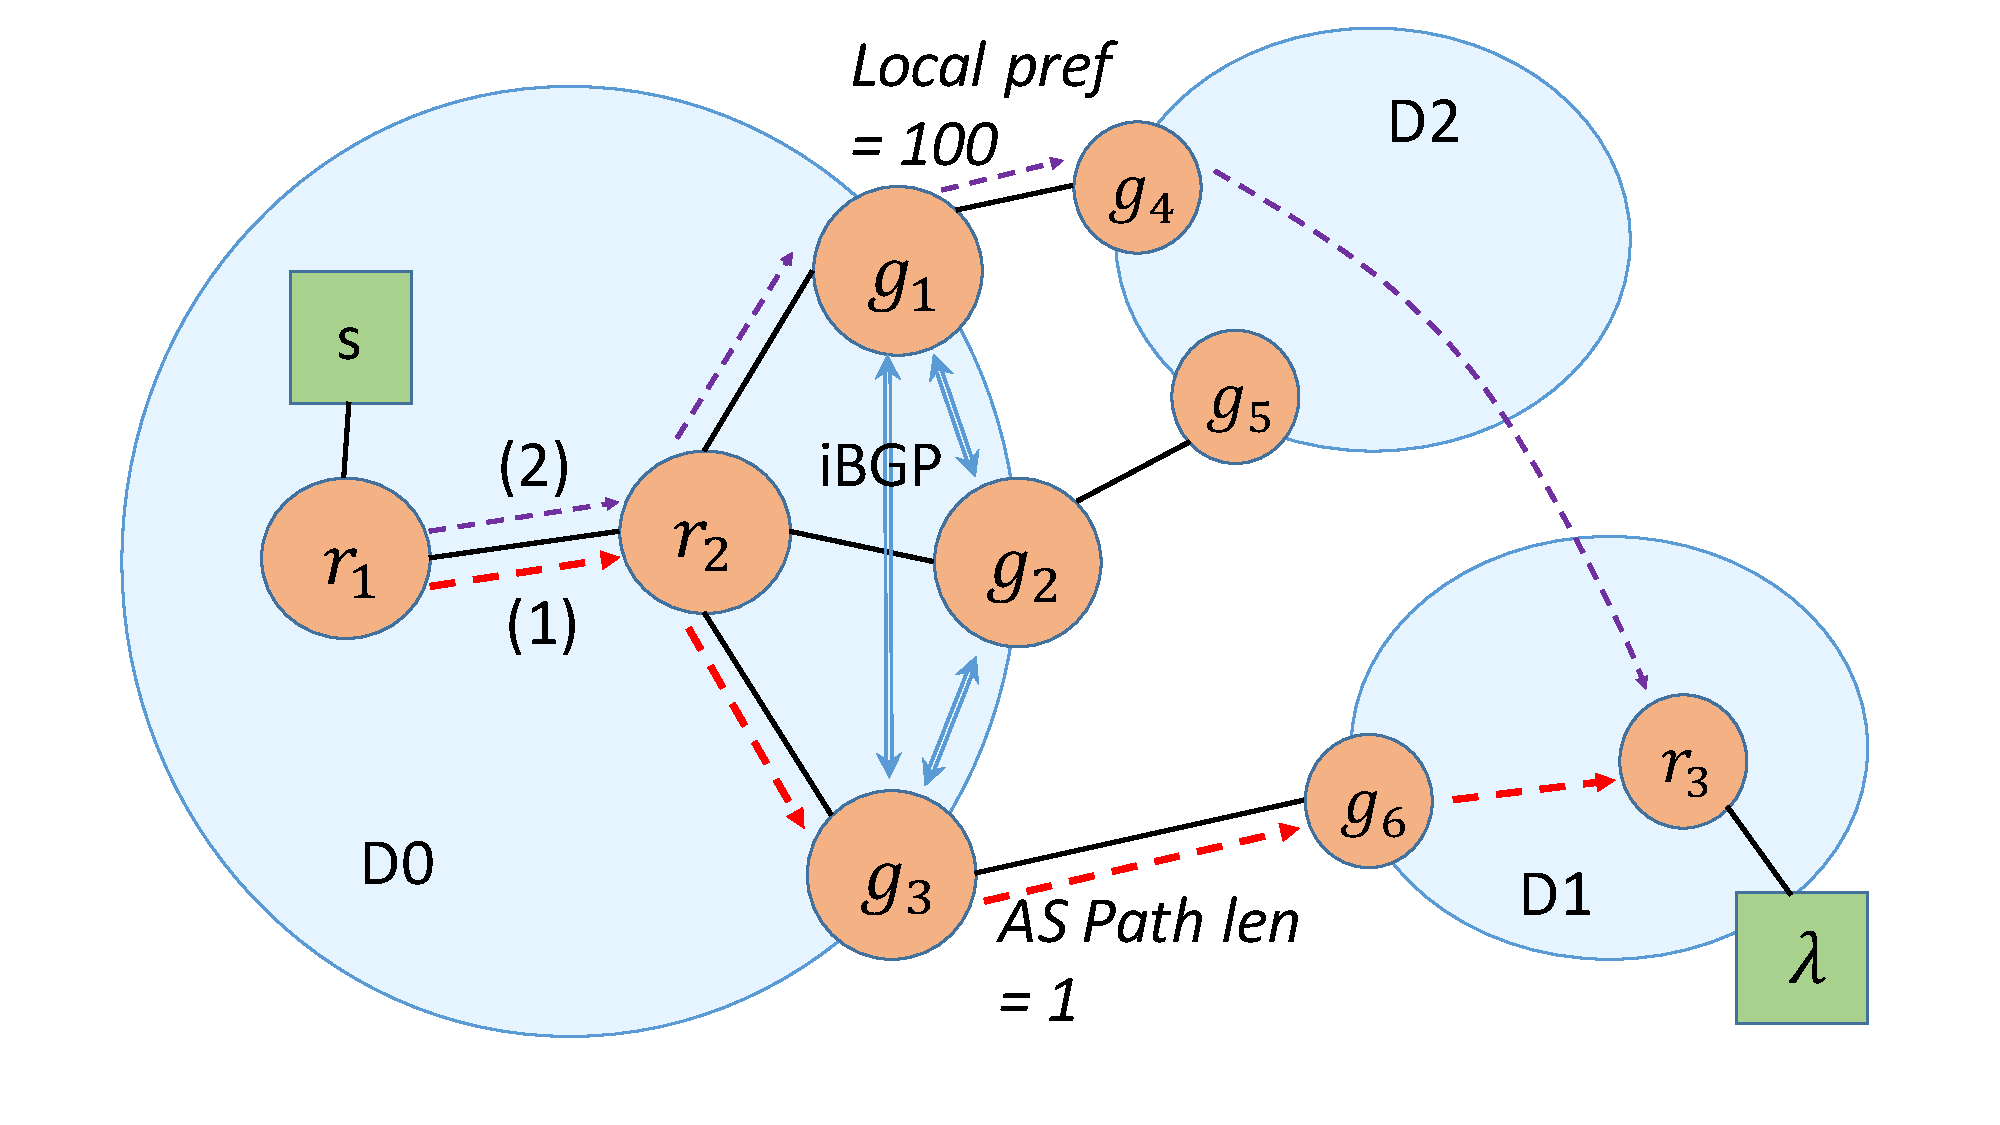
\includegraphics[width=0.66\columnwidth]{figures/bgp-example.pdf}}
	\compactcaption{\label{fig:bgpexample}
	How to configure inter-domain routing, CHANGE dst to lambda}
\end{figure*}


\subsection{BGP configuration}
In \Cref{fig:bgpeg}, we show how \name configures BGP in domain AS0 
to ensure that traffic from $src$ to $dst$ is routed across domains 
such that it follows the path $p$ provided as input. Suppose path (1) is
provided as input. G3 receives a route for $dst$ with AS path length 1
(AS2), while G1 and G2 will receive a route for $dst$ with 
AS path length 2 (AS1, AS2). Since, we need to send traffic along
G3, we do not need to configure any additional BGP variable for $dst$;
\Cref{alg:bgppathrules} will choose the best route for $dst$ 
via G3 (which is the gateway of the input path) as all routes have
the same local preference (0) and AS path length is used to  and $R1$ will
send the packet to $dst$ to G3 along the shortest path (which 
follows the subpath of $p$ from $R1$ to $G3$ by OSPF synthesis). 

Consider the example of input path (2) for $src$ to $dst$ 
in \Cref{fig:bgpeg}. Since, $G1$'s route has a longer AS 
path length greater than $G3$'s route and equal to $G2$'s route,
we need to set the local preference of route received by $G1$ 
(from $G4$) to 100 (any positive value). Thus, \Cref{alg:bgppathrules} 
will select $G1$ as the exit gateway for $dst$. The subpath
$R1$ to $G1$ will be given appropriate weights by the OSPF
synthesis phase so that the synthesizing configurations 
forward traffic along the input path. 

Suppose, traffic for $dst$ exited through two different
gateways in a domain for different paths (\Cref{fig:bgpexample}(b)).
$src1$'s traffic to $dst$ exits domain 0 through 
gateway router $G1$, while $src2$'s traffic exits 
through $G2$. Therefore, both these routes need to be 
redistributed to the OSPF domain. Therefore, we assign
$LP(G1,G2,dst) = 100$ and $LP(G2,G4,dst) = 200$. For 
router $G2$ and destination $dst$, 
no other route has a local preference value $>200$, thus 
the route along the path is chosen. However, the iBGP route
sent by $G2$ with local preference 200 will be preferred over
the $G1\rightarrow G3$ route which has local preference 100.
Thus, we add a iBGP filter for connection $G2 \rightarrow G1$ for
destination IP $dst$ ($G1$ and $G2$ need not be connected by a 
link directly; iBGP establishes a connection among the 
BGP routers in a domain). Thus, $G1$ will not receive the
$G2 \rightarrow G4$ route from $G2$, and the route $G1 \rightarrow
G3$ route would be chosen as it has the highest local preference
of all routes received by $G1$. 

\subsubsection{Static Routes} \label{sec:static}
As shown in \Cref{} (Refer to example of 
static routes in motivating example), we require static routes 
to enforce AS paths with loops. Static routes have the lowest 
administrative distance (1) by default~\cite{ad}, and will override BGP
and OSPF routes at a router, this feature can be used to 
exit and enter a domain multiple times. While static routes
do not reduce the resilience of the network (all routes are still
enabled, unlike route-filters), a network under flux will have
unpredictable routing behaviour, unlike with only OSPF and BGP
configured at the routers. 
Also, static routes have to be installed per-destination, thus increasing
the size of configurations drastically as number of policy paths increase.

Given a path $p$ for subnet $\lambda$ and 
the corresponding AS path $p_{as}
= as_1 \rightarrow as_2 \rightarrow \ldots \rightarrow as_m$ (where
$as_m = \Theta(\lambda)$), static
routes are required if $p_{as}$ has a AS-loop. 
To minimize
the number of static routes, we find 
the smallest $i \in [1,m]$ 
such that $\overline{p_{as}} = as_i \rightarrow as_{i+1}
\rightarrow \ldots \rightarrow as_m$ has no loops. 
Therefore, $\overline{p_{as}}$ is the longest AS-loop-free
subpath of $p_{as}$, and be can be enforced using BGP and OSPF. For the 
network path corresponding to AS path $as_1 \rightarrow as_2 
\rightarrow \ldots \rightarrow as_{i-1}$, we require static
routing rules for each next-hop. The static routing score
is the total number of static route hops required to enforce
the input paths.
\todo{Write about the BGP paths are extracted for the next phase}

\subsubsection{BGP Local Preference Entries}
\name uses BGP local preference to route traffic
for a particular subnet to the next AS via a specific 
gateway as per the input paths obtained. 
As shown in \Cref{} (Refer
to ex), if there are multiple exit gateways from an AS 
for a subnet $\lambda$, we require local preference entries at the 
gateways and iBGP filters among these gateways for $\lambda$.

For a domain $d$ and subnet $\lambda$, consider the set 
of paths to $\lambda$ exiting $d$ using BGP (and not statically
routed as described in \Cref{sec:static}). Let $E$ denote the
set of exit gateway routers for the paths of $\lambda$. 
If $|E| = 1$, if gateway $g$ receives a route with 
strictly shortest AS path length (\Cref{alg:bgppathrules}) 
which enforces the paths
for $\lambda$, we do not need to configure local preference
entries on any BGP router in the domain for $\lambda$. If
the exit route chosen by the gateways for $\lambda$ does not 
enforce the paths, \name configures a local preference entry
for $\lambda$ at exit gateway, and thus, the exit route chosen
by BGP enforces the input paths for $\lambda$ in the domain.

If $|E| ~> 1$, multiple BGP routes must be redistributed to 
the OSPF domain.
E local prefs + E(E - 1) iBGP filters!

\todo{Changes to OSPF synthesis to ensure closest gateway}
\subsection{Multiple Gateways}
When BGP routes to a destination $\lambda$ 
from multiple gateways are redistributed in
the OSPF domain, \name uses a modified OSPF synthesis
algorithm from \secref{sec:ospfsynthesis}. This is 
required because an OSPF router will choose
the closest BGP gateway in terms of OSPF distance 
for $\lambda$. For instance, a router $r$ will choose
from gateways $g_1$ and $g_2$ according to the $r-g_1$
and $r-g_2$ distance. Therefore, given the input path in
the domain $p=r \rightarrow^+ g1$, \name adds additional
constraints ensuring the distance to $g_2$ from routers
on the path is strictly
greater than the distance to $g_1$ 
on top of the constraints ensuring
$p$ is the shortest path from $r$ to $g_1$. 
Let us define $G_\lambda$ to be the set of gateways
for destination $\lambda$ in the domain. For 
a router $r$, $g \in G_\lambda$ is the gateway if
$r \rightarrow^+_{\xi_{\lambda}} g$ holds, i.e., $g$ 
is reachable from $r$ in the DAG $\xi_{\lambda}$.  
\name adds the following constraints to the 
OSPF synthesis phase to ensure a router
chooses the correct gateway to ensure the input 
paths are induced: 
\begin{multline} \label{eq:gateway}
\forall g \in G_{\lambda}.~\forall r \in \xi_\lambda 
\wedge r \rightarrow^+_{\xi_{\lambda}} g. \\
~\forall g' \in G_{\lambda} \wedge g' \not= g. 
~\forall n' \in N(r) \setminus N_{\xi_\lambda}(r). \\
E(r, n') + D(n', g') > \sum_{\mathclap{\substack{(r_i,r_j) \in r \rightarrow^+_{\xi_{\lambda}} g }}} 
E(r_i, r_j) 
\end{multline}
Like unmodified OSPF synthesis, the system of
constraints generated could be inconsistent and require
route-filters to eliminate constraints. In this scenario,
OSPF needs to filter shorter routes to gateways, and
thus the synthesized configuration would forward traffic to
the gateway specified by the input. We use the same 
approach of picking route-filters from the unsatisfiable core
(\secref{sec:routefilter}), route-filter $((r, n'), \lambda)$
maps to following constraint in the IIS for some $g,g'$: 
\begin{equation}
E(r, n') + D(n', g') > \sum_{\mathclap{\substack{(r_i,r_j) \in r \rightarrow^+_{\xi_{\lambda}} g }}} 
E(r_i, r_j) 
\end{equation}
\todo{abrupt}